\documentclass{article}

\usepackage{float}
\usepackage[utf8]{inputenc}
\usepackage{hyperref}
\usepackage[hyperref=true, natbib=true, style=numeric, backend=bibtex]{biblatex}
\usepackage{graphicx}
\bibliography{references.bib}

\title{TCP Congestion Algorithms In Datacenters \\
	\vspace{0.3cm}
	{\large LS Project}
}
\date{\today{}}
\author{Luc Gommans, Rick van Gorp}

\begin{document}
\maketitle

\section{Abstract}


\section{Introduction}

% Copied from proposal
% Edited 27-11-2017

Multitentant datacenters aim to provide services with consistent performance
and reliability. When customers send a lot of data in a short amount of time,
networks might become congested, which results in lowered performance.

Congestion occurs when a buffer on the path to the recipient is full and
packets are dropped. TCP has a mechanism to avoid congestion in the network:
TCP congestion control. Multiple algorithms are available for congestion
control and show a different behaviour depending on the network's
characteristics.

In 2010, the algorithm DCTCP was described in an
article\cite{dctcp-congestion-original} and published as RFC8257 in
2017\cite{dctcp-congestion}. DCTCP is optimized for datacenters and provides a
high-burst tolerance, low latency, and high throughput when the datacenter has
a small part of the buffer available\cite{dctcp-congestion}. In 2016 another
algorithm was proposed: BBR. This is a TCP congestion algorithm created by
Google, which achieves higher bandwidths and lower latencies compared to other
TCP congestion methods\cite{bbr-congestion}. A comparison of BBR with
CUBIC\cite{bbr-congestion-comparison} shows that the BBR node pushes the CUBIC
node away in bandwidth when using small buffers. The BBR node gets more
bandwidth allocated than the CUBIC node.

This report includes a performance and behavior analysis of different TCP congestion control algorithms in a (simulated) multitenant datacenter network. Based on the results, we will recommend datacenters on measures to take to keep providing a reliable environment for customers when multiple congestion control algoritms are active in the network, for example using Quality of Service or discouraging certain congestion control algorithms. The main research question is: {\it How can a datacenter provide a reliable and performant environment for customers when multiple TCP congestion control algorithms are used in the
network?}

\section{Related work}

% Copied from proposal

The TCP congestion control algorithm BBR is discussed in \cite{bbr-congestion}.
The journal contains a performance test of the BBR algorithm and a comparison
between the BBR algorithm and the CUBIC algorithm, where a noticeable
difference in bandwidth allocation is shown when using small buffers.

In \cite{multiple-congestion} a performance analysis of multiple TCP congestion
control algorithms is performed. This research does not include the new
congestion control algorithms we want to analyze and does not include the
datacenter context.

In \cite{dctcp-congestion-original} an algorithm is proposed to avoid
congestion within datacenters. The authors describe an algorithm that maintains
a small buffer occupancy and has an early detection of congestion.

\section{Method}
During this research a performance test of various TCP congestion algorithms will be performed. The most common TCP congestion algorithms will be determined through desk research. The tests will be conducted in a private environment. Based on the results of those tests, recommendations will be given related to the measures a datacenter has to take to keep the traffic equally allocated over customers. 

	\subsection{Selecting TCP congestion algorithms}	
	In order to select the most common TCP congestion algorithms desk research will be performed. Results of scientific reports will show which algorithms are used more often than other algoritms. Based on those results a list of TCP congestion algorithms will be composed.	
	
	\subsection{Comparing Performance}
	One scenario will be used to compare the performance of the TCP congestion algorithms:
	\begin{enumerate}
		\item The user owns multiple endpoints in the network. In this case a congestion algorithm is applied at both the client and server side. This scenario applies to multitentant datacenter situations, where a user owns a server in the datacenter network and a node outside of the datacenter network.
	\end{enumerate}
	
	The created environment is shown in figure \ref{fig:setup1}.

	\begin{figure}[H] 
		\centering
  			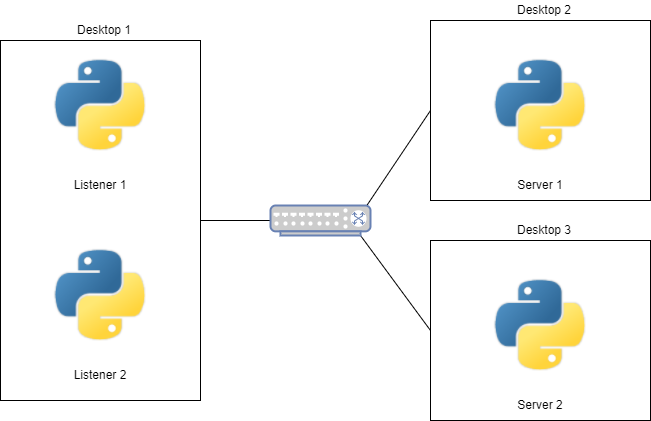
\includegraphics[scale=0.5]{figs/setup2.png}
  			\caption{Test setup - Scenario 1}
  		\label{fig:setup1}
	\end{figure}
	
	In scenario 1 the user server uses the same algorithm as the user node and the random server uses the same algorithm as the random node. Tests in this scenario cover behavioral differences between TCP congestion algorithms when a user owns a node in the network of a multitenant datacenter.
	
	In both scenarios the TCP congestion algorithms are tested for multiple characteristics:
	\begin{enumerate}
		\item TCP Window Size measured over time: to determine whether using a specific TCP congestion algorithm in combination with other TCP congestion algorithms results in the allocation of a larger window or a smaller window to a specific TCP connection.
		\item Bandwidth allocation: to determine whether using a specific TCP congestion algorithm in combination with other TCP congestion algorithms results in the allocation of more bandwidth to a specific TCP connection.
		\item Round Trip Time: to determine the reason of the behaviour of a TCP congestion algorithm in combination with other TCP congestion algorithms.
	\end{enumerate}
The tests conducted on the algorithms have two environment variables: packet loss and delay. Those environment variables are simulated using \texttt{netem}, which is a network emulation functionality in several Linux distributions \cite{linux-netem}. Packet loss and delay are chosen as the behavior of most TCP algorithms depend on those variables [SRC]. The values for the environment variables are chosen based on measurements performed by Verizon \cite{verizon-latency}.

		\subsubsection{Determining the Packet loss and Delay}
		The dataset of Verizon \cite{verizon-latency} is used to calculate the packet loss and delay used in this research. The dataset includes global information and shows averages per month over the year 2017. The packet loss is calculated by taking the average of the Verizon Business Packet Delivery Statistics for Country Specific Metrics for each country. Those averages were inverted by subtracting the packet delivery percentage from 100, to show the actual packet loss in percentages and not the packet delivery. Based on the ascending sorted values a bar chart was created. This bar chart is shown in figure \ref{fig:packet-loss-chart}
		
	\begin{figure}[H] 
		\centering
  			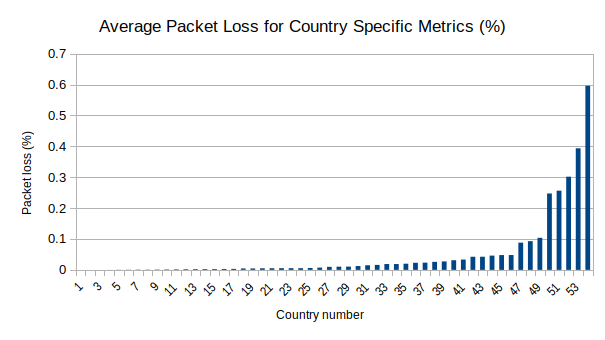
\includegraphics[scale=0.7]{figs/verizon-packetloss.png}
  			\caption{Average Packet Loss for Country Specific Metrics}
  		\label{fig:packet-loss-chart}
	\end{figure}

The country numbers in figure \ref{fig:packet-loss-chart} are only used to show the distribution of the average packet loss. The maximum packet loss shown in figure \ref{fig:packet-loss-chart} equals 0.6\% and the minimum equals 0\%. However, in case of situations where more packet loss occurs than usual, the double value of the maximum is used: 1.2\%. The values for packet loss in this comparison set-up were determined based on the distribution shown in figure \ref{fig:packet-loss-chart} and the manually set maximum of 1.2\%. The values are shown in table \ref{table:test-packetloss}.	
	
	\begin{table}[H]
		\centering
		\caption{Packet loss percentages used for the comparison setup}
		\begin{tabular}[H]{ | l |}
		\hline
		\textbf{Packet loss} \\
		\hline 0\%. \\
		\hline 0.01\% \\
		\hline 0.1\% \\
		\hline 0.6\% \\
		\hline 1.2\% \\
		\hline
		\end{tabular}
		\label{table:test-packetloss}
	\end{table}

The delay is calculated by taking the average of the Verizon Business Latency Statistics for Country Specific Metrics for each country. Based on the ascending sorted values a bar chart was created. This bar chart is shown in figure \ref{fig:verizon-delay-chart}

	\begin{figure}[H] 
		\centering
  			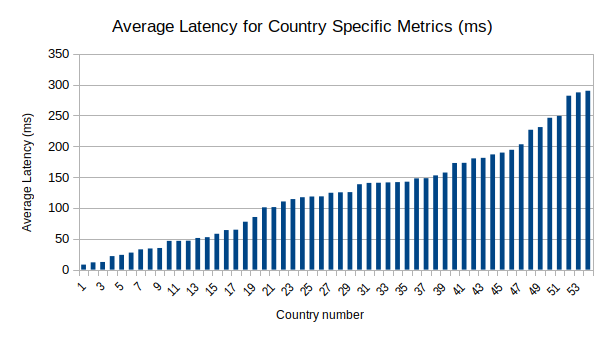
\includegraphics[scale=0.7]{figs/verizon-delay.png}
  			\caption{Average Latency for Country Specific Metrics}
  		\label{fig:verizon-delay-chart}
	\end{figure}
	
The country numbers in figure \ref{fig:verizon-delay-chart} are only used to show the distribution of the average delays. The maximum delay shown in figure \ref{fig:verizon-delay-chart} equals 290ms and the minimum equals 8ms (both rounded). The values for delay in this comparison set-up were determined based on the distribution shown in figure \ref{fig:verizon-delay-chart}. The values are shown in table \ref{table:test-delay}.	
	
	\begin{table}[H]
		\centering
		\caption{Packet loss percentages used for the comparison setup}
		\begin{tabular}[H]{ | l |}
		\hline
		\textbf{Delay} \\
		\hline  8ms\\
		\hline  64ms  \\
		\hline  120ms  \\
		\hline  176ms \\
		\hline	232ms \\
		\hline  290ms  \\
		\hline
		\end{tabular}
		\label{table:test-delay}
	\end{table}

		\subsubsection{Performing time-based automated tests}
		The tests will be performed using scripts written in Python [\ref{appendix:python}]. The scripts either act as controller or as disciple. The controller is responsible for controlling the tests, by synchronizing the time, exchanging commands to run, modify or stop the tests and gathering data. The disciple is the listener and executes all task commands the controller sends. The commands include getting the hostname of a disciple, setting the TCP congestion algorithm of a disciple, configuring the time of a disciple, starting the data transfer from a disciple and closing the connection with the controller.

		\subsubsection{Testing hardware}
		The specifications of the hardware used for the tests are shown in table \ref{table:spec1}, table \ref{table:spec2} and table \ref{table:spec3}. The switch shown in table \ref{table:spec3} has all router related functionalities, which might impact the network speed, turned off.

		\begin{table}[H]
			\centering
			\caption{Node configurations}
			\begin{tabular}[H]{ | l | l | }
			\hline
			\textbf{Hardware} & \textbf{Specification} \\
			\hline  Model & Dell Optiplex 7010\\
			\hline  CPU & Intel(R) Core(TM) i5-3570S CPU @ 3.10GHz\\
			\hline  Memory & 12GB\\
			\hline  NIC & Intel Corporation 82579LM Gigabit Network Connection (rev 04)\\
			\hline	NIC Driver & e100e 3.2.6-k\\
			\hline
			\end{tabular}
			\label{table:spec1}
		\end{table}

		\begin{table}[H]
			\centering
			\caption{Switch 1 configuration}
			\begin{tabular}[H]{ | l | l | }
			\hline
			\textbf{Hardware} & \textbf{Specification} \\
			\hline  Model & 3Com OfficeConnect Gigabit Switch 16\\
			\hline  Ports & 16x Gigabit Ethernet\\
			\hline
			\end{tabular}
			\label{table:spec2}
		\end{table}
		
		\begin{table}[H]
			\centering
			\caption{Switch 2 configuration}
			\begin{tabular}[H]{ | l | l | }
			\hline
			\textbf{Hardware} & \textbf{Specification} \\
			\hline  Model & Sitecom Gigabit Router 300N-XR\\
			\hline  Ports & 4x Gigabit Ethernet\\
			\hline
			\end{tabular}
			\label{table:spec3}
		\end{table}

	\subsection{Traffic Management}
	Desk research will be conducted to gather information related to traffic management. The goal is to find a mechanism that is capable of allocating bandwidth equally between customers of a datacenter. This is done by analyzing the results from the algorithm comparison and the initial desk research on traffic management. 

\section{Results}
Type some text here.

	\subsection{TCP Congestion Algorithms}
	The most common TCP congestion algorithms are CTCP, CUBIC and BIC. CTCP is the default congestion algorithm in Microsoft Windows Server 2008 and newer \cite{cubic-kernel-version}. CUBIC is the default congestion algorithm in Linux distributions with kernel versions 2.6.19 and higher \cite{cubic-kernel-version}. BIC was the default congestion algorithm in earlier Linux distributions from kernel version 2.6.8 until 2.6.19 \cite{bic-kernel-version} \cite{cubic-kernel-version}. DCTCP and BBR will also be tested as those protocols are newer. DCTCP is specifically designed for datacenters \cite{dctcp-congestion} and BBR is a new congestion protocol not yet widely deployed \cite{bbr-congestion}.
	
		\subsubsection{Algorithm Characteristics}
		- Includes characteristics of the algorithms. To what do the TCP congestion algorithms respond according to literature? And how do they deal with that (If available in literature).
		
		\subsubsection{Performance comparison}	
		- Includes results of tests.
	
	\subsection{Traffic Management}
	- Includes what is available for trafic management in a datacenter.
	- Measures to take to equally allocate bandwidth to customers.
		\subsubsection{Quality of Service}
			
		
		

\section{Discussion}


\section{Conclusion}

% For reference, from the proposal:

Our main research question is:
{\it How can a datacenter provide an reliable and performant environment for
customers when multiple TCP congestion control algorithms are used in the
network?}

\vspace{0.5cm}

This main research question divides in five sub-questions:

\begin{enumerate}
	\item What TCP congestion algorithms are most commonly implemented?
	\item How do these TCP congestion algorithms work?
	\item How do these TCP congestion algorithms differ in behavior?
	\item What is the impact on the availability and service for customers when using different, competing congestion algorithms?
	\item What measures could be taken to split bandwidth equally among tenants?
\end{enumerate}


\printbibliography

\appendix
\section{Python}
\label{appendix:python}
SCRIPT

\end{document}

